\documentclass[12pt]{article}
\usepackage{amsthm,amssymb,amsfonts,amsmath,amstext,systeme}
\usepackage{graphicx,float}
\marginparwidth 0pt
\oddsidemargin -1.2 truecm
\evensidemargin  0pt 
\marginparsep 0pt
\topmargin -2.2truecm
\linespread{1}
\textheight 25.8 truecm
\textwidth 18.5 truecm
\newenvironment{remark}{\noindent{\bf Remark }}{\vspace{0mm}}
\newenvironment{remarks}{\noindent{\bf Remarks }}{\vspace{0mm}}
\newenvironment{question}{\noindent{\bf Question }}{\vspace{0mm}}
\newenvironment{questions}{\noindent{\bf Questions }}{\vspace{0mm}}
\newenvironment{note}{\noindent{\bf Note }}{\vspace{0mm}}
\newenvironment{summary}{\noindent{\bf Summary }}{\vspace{0mm}}
\newenvironment{back}{\noindent{\bf Background}}{\vspace{0mm}}
\newenvironment{conclude}{\noindent{\bf Conclusion}}{\vspace{0mm}}
\newenvironment{concludes}{\noindent{\bf Conclusions}}{\vspace{0mm}}
\newenvironment{dill}{\noindent{\bf Description of Dill's model}}{\vspace{0mm}}
\newenvironment{maths}{\noindent{\bf Mathematics needed}}{\vspace{0mm}}
\newenvironment{inst}{\noindent{\bf Instructions}}{\vspace{0mm}}
\newenvironment{notes}{\noindent{\bf Notes }}{\vspace{0mm}}
\newenvironment{theorem}{\noindent{\bf Theorem }}{\vspace{0mm}}
\newenvironment{example}{\noindent{\bf Example }}{\vspace{0mm}}
\newenvironment{examples}{\noindent{\bf Examples }}{\vspace{0mm}}
\newenvironment{topics}{\noindent{\bf Topics}}{\vspace{0mm}}
\newenvironment{outcomes}{\noindent{\bf Expected Learning Outcomes}}{\vspace{0mm}}
\newenvironment{lemma}{\noindent{\bf Lemma }}{\vspace{0mm}}
\newenvironment{solution}{\noindent{\it Solution}}{\vspace{2mm}}
\newcommand{\ds}{\displaystyle}
\newcommand{\un}{\underline}
\newcommand{\bs}{\boldsymbol}

\begin{document}

\baselineskip 18 pt
\begin{center}
	{\large \bf HKDSE MATH M2 2023}\\
	\vspace{2 mm}

\end{center}
\vspace{0.05cm}

\begin{enumerate}
	\item \textbf{HKDSE Math M2 2023 Q1}\\
	Let $a$ be a constant. If the coefficient of $x$ in the expansion of $(2-3x)^5\left(x + \dfrac{a}{x}\right)^2$ is $\dfrac{160}{3}$, find $a$ and the coefficient of $x^2$ in the expansion.\\
	(5 marks)

	\item \textbf{HKDSE Math M2 2023 Q2}\\
	Let $f(x) = -x \sin{x}$.
	\begin{enumerate}
		\item [(a)]Prove that $f\left(\dfrac{\pi}{2} + h\right) - f\left(\dfrac{\pi}{2}\right) = \pi \sin^2{\left(\dfrac{h}{2}\right)} - h \cos{h}$.
		\item [(b)]Using (a), find $f'\left(\dfrac{\pi}{2}\right)$ from the first principles.
	\end{enumerate}
	(5 marks)

	\item \textbf{HKDSE Math M2 2023 Q3}
	\begin{enumerate}
		\item [(a)]Find a pair of constants $p$ and $q$ such that $$11\sin{x} + 7\cos{x} \equiv p(3\sin{x} + \cos{x}) + q(3\cos{x} - \sin{x}).$$
		\item [(b)]Evaluate $\displaystyle \int^{\frac{\pi}{4}}_{0} \dfrac{11\sin{x} + 7\cos{x}}{3\sin{x} + \cos{x}} \,dx$.
	\end{enumerate}
	(6 marks)


	\item \textbf{HKDSE Math M2 2023 Q4}
	\begin{enumerate}
		\item[(a)]Prove that $\cos{3x} = 4\cos^3{x} - 3\cos{x}$.
		\item[(b)]Using (a), solve the equation $\sec^3{x} - 6\sec^2{x} + 8 = 0$, where $\dfrac{\pi}{2} < x < \dfrac{3\pi}{2}$.
	\end{enumerate}
	(5 marks)

	\item \textbf{HKDSE Math M2 2023 Q5}\\
	Let $A$ be $2\times2$ real matrix such that $A^2 + A + I = 0$, where $I$ is the $2\times2$ identity matrix. 
	\begin{enumerate}
		\item [(a)]Prove that $A^3 = I$.
		\item [(b)]Prove that $A$ is non-singular.
		\item [(c)]Someone claims that $\left(A^{1000} + (A^{-1})^{2000}\right)^{-1}$ can be expressed in the form of $\alpha I + \beta A$, where $\alpha$ and $\beta$ are real numbers. Is the claim correct? Explain your answer.
	\end{enumerate}
	(7 marks)


	\item \textbf{HKDSE Math M2 2023 Q6}
	\begin{enumerate}
		\item [(a)]Let $r$ be a positive constant. Figure 1 shows the shaded region which is inside the circle $x^2 + (y-r)^2 = r^2$ and below the horizontal line $y = h$, where $0 \leq h \leq 2r$. Prove that the volume of the solid of revolution generated by revolving the shaded region about the $y$-axis is $\dfrac{\pi}{3}h^2(3r-h)$.
		\begin{figure}[H]
			\centering
			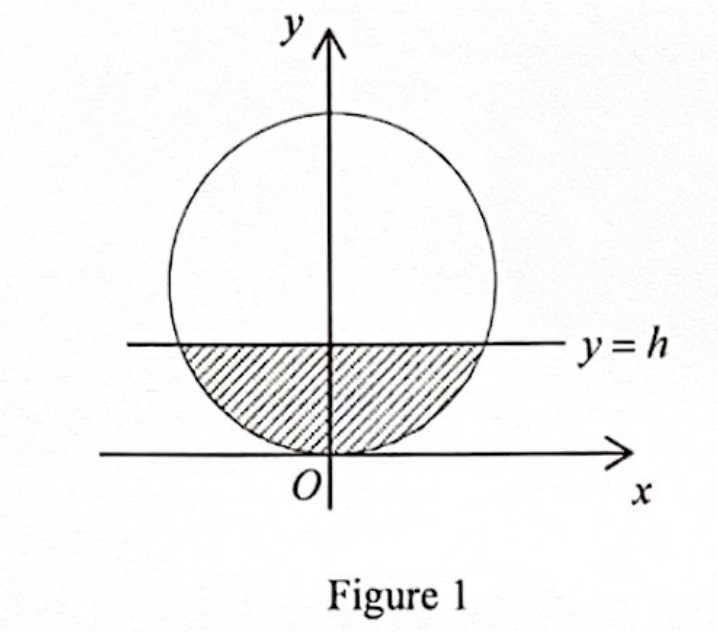
\includegraphics[width = .5\linewidth]{2023Figure1}
		\end{figure}
		\item [(b)]A solid metal sphere of radius 10 cm is put into an empty right cylindrical container of radius 11 cm and height 20 cm, with longitudinal section as shown in Figure 2. Starting from time $t=0$, water is added to the container at a constant rate of 1 cm$^3$ per second. Let $h$ cm be the depth of water after $t$ seconds. By expressing $\dfrac{\text{d}h}{\text{d}t}$ in terms of $h$, find the greatest value of $\dfrac{\text{d}h}{\text{d}t}$.
		\begin{figure}[H]
			\centering
			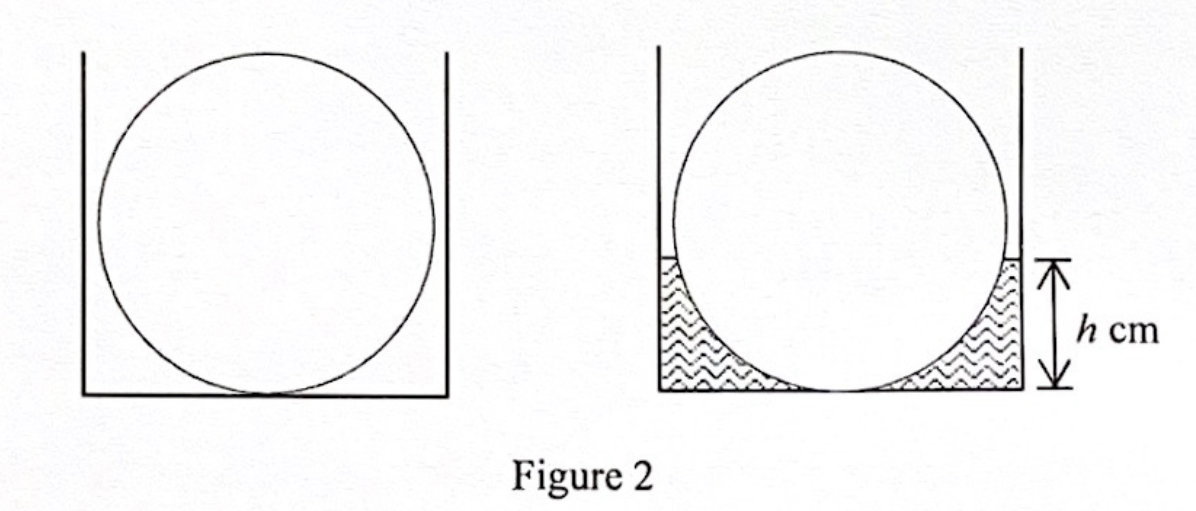
\includegraphics[width = .5\linewidth]{2023Figure2}
		\end{figure}
	\end{enumerate}
	(7 marks)

	\item \textbf{HKDSE Math M2 2023 Q7}\\
	Let $f(x)$ be a function defined on the interval $(-2,2)$. Denote the curve $y = f(x)$ by $\Gamma$. At any point $(x,y)$ on $\Gamma$, the slope of the tangent to $\Gamma$ is $\dfrac{k - 3x}{\sqrt{4-x^2}}$, where $k$ is a constant. It is given that $\Gamma$ passes through the origin.
	\begin{enumerate}
		\item [(a)]Find the equation of $\Gamma$ in terms of $k$.
		\item [(b)]Suppose that $\Gamma$ has a turning point.
		\begin{enumerate}
			\item [(i)]Find the range of values of $k$.
			\item [(ii)]Does $\Gamma$ have a point of inflexion? Explain your answer.
		\end{enumerate}
	\end{enumerate}
	(7 marks)

	\item \textbf{HKDSE Math M2 2023 Q8}
	\begin{enumerate}
		\item [(a)]Let $\theta \in \mathbb{R}$. Using mathematical induction, prove that $\displaystyle \sin{\theta}\sum_{k=1}^{n}\sin{2k\theta} = \sin{n\theta}\sin{(n+1)\theta}$ for all positive integers $n$.
		\item [(b)] Using (a), find a pair of rational numbers $a$ and $b$ such that $\displaystyle\sum_{k = 1}^{111}\sin{\dfrac{k\pi}{11}}\cos{\dfrac{k\pi}{11}} = a\sin{b\pi}$, where $0 < b < \dfrac{1}{2}$.
	\end{enumerate}
	(8 marks)

	\item \textbf{HKDSE Math M2 2023 Q9}\\
	Define $ f(x) = xe^{-x^2}$ for all $x\in \mathbb{R}$. Denote the graph of $y = f(x)$ by $G$.
	\begin{enumerate}
		\item [(a)]Find $f'(x)$ and $f''(x)$. \\(3 marks)
		\item [(b)]Find the maximum point(s) and minimum point(s) of $G$. \\(3 marks)
		\item [(c)]Let $L$ be the tangent to $G$ at the point $\left(1,\dfrac{1}{e}\right)$.
		\begin{enumerate}
			\item [(i)]Find the equation of $L$.
			\item [(ii)]By considering $f''(x)$, explain why $G$ lies below $L$ in the interval $(0,1)$.
			\item [(iii)]Find the area of the region bounded by $G$, $L$ and the $y$-axis.
		\end{enumerate}
		(6 marks)
	\end{enumerate}

	\item \textbf{HKDSE Math M2 2023 Q10}\\
	Let $O$ be the origin. The position vectors of $P$ and $Q$ are $-2\textbf{i} - \textbf{k}$ and $2\textbf{i} -\textbf{j}+ \textbf{k}$ respectively. Denote the circle passing through $O$, $P$ and $Q$ by $C$. Let $R$ be a point lying on $PQ$ such that $OR$ is perpendicular to $OQ$.
	\begin{enumerate}
		\item [(a)] By considering the ratio of $PR$ to $RQ$, find $\overrightarrow{OR}$. \\(3 marks)
		\item [(b)] $OR$ produced meets $C$ at another point $S$. Find $\overrightarrow{OS}$. \\(3 marks)
		\item [(c)] Let $\Pi$ be the plane which contains $C$.
		\begin{enumerate}
			\item [(i)] Find a non-zero vector which is perpendicular to $\Pi$.
			\item [(ii)] Let $G$ be the center of $C$. Denote the projection of point $A(-6, -22,2)$ on $\Pi$ by $B$. Describe the geometric relationship between $O$, $B$ and $G$. Explain your answer.
		\end{enumerate}
		(6 marks)
	\end{enumerate}

	\item \textbf{HKDSE Math M2 2023 Q11}
	\begin{enumerate}
		\item [(a)] Consider the system of linear equations in real variables $x$, $y$, $z$
		$$(E) : \left\{\begin{matrix}
		x&	+&	ay&		+&	(a+1)z&		=&	2  \\
		x&	+&	(a+4)y&	+&	(2a+4)z&	=&	b+1 \\
		2x&	+&	3y&		+&	5z&			=&	b \\
		\end{matrix}\right. \text{,  where } a, b \in \mathbb{R} .$$
		\begin{enumerate}
			\item [(i)] Assume that $(E)$ has a unique solution. Find the range of values of $a$.
			\item [(ii)] Assume that $a = 1$. If $(E)$ is consistent, find $b$.
			\item [(iii)] Assume that $a \neq 1$ and $(E)$ is incnsistent. Find the range of values of $b$.
		\end{enumerate}
		(7 marks)
		\item [(b)] Consider the system of linear equations in real variables $x$, $y$, $z$
		$$(F) : \left\{\begin{matrix}
		x&	+&	2y&	+&	3z&	=&	2  \\
		x&	+&	6y&	+&	8z&	=&	s+1 \\
		2x&	+&	3y&	+&	5z&	=&	s \\
		\end{matrix}\right. \text{,  where } s \in \mathbb{R} .$$
		Does there exist a pair of real constants $m$ and $n$ (independent of $s$) such that for every $s\in\mathbb{R}$, $(F)$ has a real solution $(x,y,z)$ satisfying $mx + ny + z = -2$? Explain your answer. \\(6 marks) 
	\end{enumerate}



	\item \textbf{HKDSE Math M2 2023 Q12}
	\begin{enumerate}
		\item [(a)]Let $a$ be a non-zero constant. Prove that $\displaystyle \int _{0}^{1} x^2e^{ax} \,dx = \dfrac{(a^2 - 2a + 2)e^a - 2}{a^3}$. \\(3 marks)		
		\item [(b)]Using (a) and integration by substitution, evaluate $\displaystyle \int _{0}^{e-1} x(\ln{(1+x)})^2 \,dx $. \\(4 marks)		
		\item [(c)]Evaluate $\displaystyle \int _{0}^{\frac{\pi}{2}} (\ln{(1+(e-1)\cos{x})})^2\sin{2x} \,dx $. \\(3 marks)
		\item [(d)]Evaluate $\displaystyle \int _{\frac{\pi}{2}}^{\pi} (\ln{(1+(e-1)\sin{x})})^2\sin{2x} \,dx $. \\(3 marks)

	\end{enumerate}




\end{enumerate}
\end{document}